\documentclass[12pt,nonacm,acmlarge,titlepage,screen]{acmart}

\def\docTitle{LaTeX Examples}
\def\docAuthor{Pierre \textsc{Le Bras}}

%% This file contains extra packages to use on top of the ACM template

%% STYLING ToC
\usepackage{titletoc}

%% SUB-FIGURES
\usepackage{subcaption}

%% ALGORITHMS
\usepackage{algorithm}
\usepackage{algorithmicx}
\usepackage{algpseudocode}

%% MORE EQUATIONS TOOLS
\usepackage{amsmath,mathtools}

%% CODE LISTINGS
\usepackage{listings}

% EASIER CROSS-REFERENCES
\usepackage[capitalise,nameinlink,noabbrev]{cleveref}

% TO GET ORDINAL NUMBERS
\usepackage[super]{nth}

\usepackage{pdflscape} % for landscape pages
\usepackage{array} % for more table options
% formatting and package settings


% document details
\def\docDate{\nth{\the\day}~\ifcase\the\month\or
  January\or February\or March\or April\or May\or June\or
  July\or August\or September\or October\or November\or
  December\fi~\the\year}
\def\docInstitution{Heriot-Watt University}
\def\docSchool{School of Mathematical and Computer Sciences}
\author{\docAuthor}
\title{\docTitle}
\date{\docDate}

% change geometry of ACM template
\geometry{twoside=true, head=13pt, foot=2pc,
     paperwidth=21cm, paperheight=29.7cm,
     includeheadfoot,
     top=78pt, bottom=114pt, inner=81pt, outer=81pt,
     marginparwidth=4pc,heightrounded
 }%

% to make sections start on new pages
% \AddToHook{cmd/section/before}{\newpage}

% colors
% main text
\def\textColor{\color[HTML]{212121}} 
\def\secTextColor{\color[HTML]{424242}}
% footer and header
\def\headerColor{\color[HTML]{565656}} 
% title, chapters, sections
\def\titleColor{\color[HTML]{212121}}

% set line spacing
% \onehalfspacing
% \singlespacing

% set table cells padding
\def\arraystretch{1.5}

% set headings format
% unset to follow ACM format
% \titleformat{\chapter}{\singlespacing\normalfont\huge\bfseries\titleColor}{\chaptertitlename\ \thechapter}{1em}{}
% \titleformat{\chapter}{\singlespacing\normalfont\huge\bfseries\titleColor}{\thechapter}{1em}{}
% \titleformat{\section}{\singlespacing\normalfont\large\bfseries\titleColor}{\thesection}{1em}{}
% \titleformat{\subsection}{\singlespacing\normalfont\large\bfseries}{\thesubsection}{1em}{}
% \titleformat{\subsubsection}{\singlespacing\normalfont\normalsize\bfseries}{\thesubsubsection}{1em}{}
% \titlespacing*{\chapter}{0pt}{0pt}{10pt}

% set paragraph indent
% unset to follow ACM format
% \setlength{\parindent}{18pt} 

% set the text colour
% \textColor 

% set hyperlinks + pdf metadata
\hypersetup{
    pdftitle={\docTitle},
    pdfauthor={\docAuthor},
    pdfkeywords={computer science dissertation},
    colorlinks=true,%
    citecolor=[HTML]{152845},%
    linkcolor=[HTML]{152845},%
    urlcolor=[HTML]{1976D2}
}

% styling the code listings
\definecolor{codegreen}{rgb}{0,0.6,0}
\definecolor{codegray}{rgb}{0.5,0.5,0.5}
\definecolor{codepurple}{rgb}{0.58,0,0.82}
\definecolor{backcolour}{rgb}{0.95,0.95,0.92}

\lstdefinestyle{mystyle}{
    backgroundcolor=\color{backcolour},   
    commentstyle=\color{codegreen},
    keywordstyle=\color{magenta},
    numberstyle=\tiny\color{codegray},
    stringstyle=\color{codepurple},
    basicstyle=\ttfamily\singlespacing,
    breakatwhitespace=false,         
    breaklines=true,                 
    captionpos=b,                    
    keepspaces=true,                 
    numbers=left,                    
    numbersep=5pt,                  
    showspaces=false,                
    showstringspaces=false,
    showtabs=false,                  
    tabsize=2
}
\lstset{style=mystyle}

% reset names for code listing
\renewcommand{\lstlistingname}{Code Listing}
\renewcommand{\lstlistlistingname}{List of \lstlistingname s}

% set cref for listing
\crefname{lstlisting}{\lstlistingname}{\lstlistingname s}
\Crefname{lstlisting}{\lstlistingname}{\lstlistingname s}

% set cross-references labels with cleveref
\crefname{appendixchapter}{Appendix}{Appendices}
\Crefname{appendixchapter}{Appendix}{Appendices}


% set custom headers/footers
% unset to follow ACM template
% \pagestyle{fancy}
% \fancyhf{}
% \renewcommand{\headrulewidth}{0pt}
% \renewcommand{\footrulewidth}{0pt}
% \fancyhead[R]{\headerColor \docType}
% \fancyhead[L]{\headerColor \docAuthor}
% \fancyfoot[C]{\headerColor \thepage}
% % Redefine the plain page style for chapter pages
% \fancypagestyle{plain}{%
%     \fancyhf{}%
%     \fancyfoot[C]{\headerColor \thepage}
% }

% custom section heading for front-matter content with addition to the ToC
\newcommand{\frontmattersection}[2]{
    \thispagestyle{plain} % remove the header on page
    % \vspace*{1cm} % to align vertically
    \phantomsection
    \begin{center} 
        \textsc{#1} 
        \addcontentsline{toc}{section}{#1}
    \end{center}
    #2 % Main Text
    \clearpage % leave blank space underneath
}

\renewcommand{\abstract}[1]{
    \frontmattersection{Abstract}{#1}
}

\newcommand{\acknowledgements}[1]{
    \frontmattersection{Acknowledgements}{#1}
}

% formatting the table of content
\dottedcontents{section}[1em]{\bfseries}{1.2em}{0pc}
\dottedcontents{subsection}[3em]{}{2.2em}{1pc}

\renewcommand{\contentsname}{Table of Contents}

% show quote marks correctly in verbatim
\usepackage{upquote}
% fancy verbatim
\usepackage{fancyvrb}
% remove headers
\fancyhead[R]{}
\fancyhead[L]{}

\begin{document}

\begin{center}
    {\Huge \textbf{\LaTeX\ Examples}}
\end{center}
\vspace{2cm}

\noindent \textbf{Author}: \docAuthor

\noindent \textbf{Date}: \nth{8} September 2025

\noindent This document contains a list of examples on how to use \LaTeX\ when you write your dissertation.

You may also check the \href{https://www.overleaf.com/learn}{Overleaf guides}.

\section*{Text}

First paragraph without indentation. 

More paragraphs with indentation.

% a comment that won't appear in the PDF

Paragraph with \textbf{bold text} and \textit{italic text}.

Paragraph with ``quotes''.

Paragraph with a url: \href{https://www.example.com/}{example.com}

Paragraph with a footnote\footnote{Footnote with extra details}.
~\\

\noindent\LaTeX:
\begin{Verbatim}[frame=single]
First paragraph without indentation. 

More paragraphs with indentation.

% a comment that won't appear in the PDF

Paragraph with \textbf{bold text} and \textit{italic text}.

Paragraph with ``quotes''.

Paragraph with a url: \href{https://www.example.com/}{example.com}

Paragraph with a footnote\footnote{Footnote with extra details}.
\end{Verbatim}

\section*{Document Structure}

% using minipage to avoid pagebreak
\noindent\begin{minipage}[t]{\textwidth}
\section{Section}
Text1
\subsection{Subsection}
Text2
\subsubsection{Subsubsection}
Text3
\paragraph{Paragraph}
Text4
\end{minipage}~\\

\noindent\LaTeX:
\begin{Verbatim}[frame=single]
\section{Section}
Text1
\subsection{Subsection}
Text2
\subsubsection{Subsubsection}
Text3
\paragraph{Paragraph}
Text4
\end{Verbatim}

\section*{Lists}

\subsection*{Bullet list}

\begin{itemize}
    \item Item 1
    \item Item 2
    \item[$\checkmark$] Item 3 
\end{itemize}

\noindent\LaTeX:
\begin{Verbatim}[frame=single]
\begin{itemize}
    \item Item 1
    \item Item 2
    \item[$\checkmark$] Item 3 
\end{itemize}
\end{Verbatim}

\subsection*{Numbered list}

\begin{enumerate}
    \item Item 1
    \item Item 2
    \item[$\star$] Item 3
\end{enumerate}

\noindent\LaTeX:
\begin{Verbatim}[frame=single]
\begin{enumerate}
    \item Item 1
    \item Item 2
    \item[$\star$] Item 3
\end{enumerate}
\end{Verbatim}

\subsection*{Nested lists}

\begin{itemize}
    \item Item 1
    \begin{itemize}
        \item Item 1
        \begin{itemize}
            \item Item 1
        \end{itemize}
    \end{itemize}
\end{itemize}
\begin{enumerate}
    \item Item 1
    \begin{enumerate}
        \item Item 1
        \begin{enumerate}
            \item Item 1
        \end{enumerate}
    \end{enumerate}
\end{enumerate}

\noindent\LaTeX:
\begin{Verbatim}[frame=single]
\begin{itemize}
    \item Item 1
    \begin{itemize}
        \item Item 1
        \begin{itemize}
            \item Item 1
        \end{itemize}
    \end{itemize}
\end{itemize}
\begin{enumerate}
    \item Item 1
    \begin{enumerate}
        \item Item 1
        \begin{enumerate}
            \item Item 1
        \end{enumerate}
    \end{enumerate}
\end{enumerate}
\end{Verbatim}

\section*{Images}

\subsection*{Single image}

\begin{figure}[ht]
    \centering
    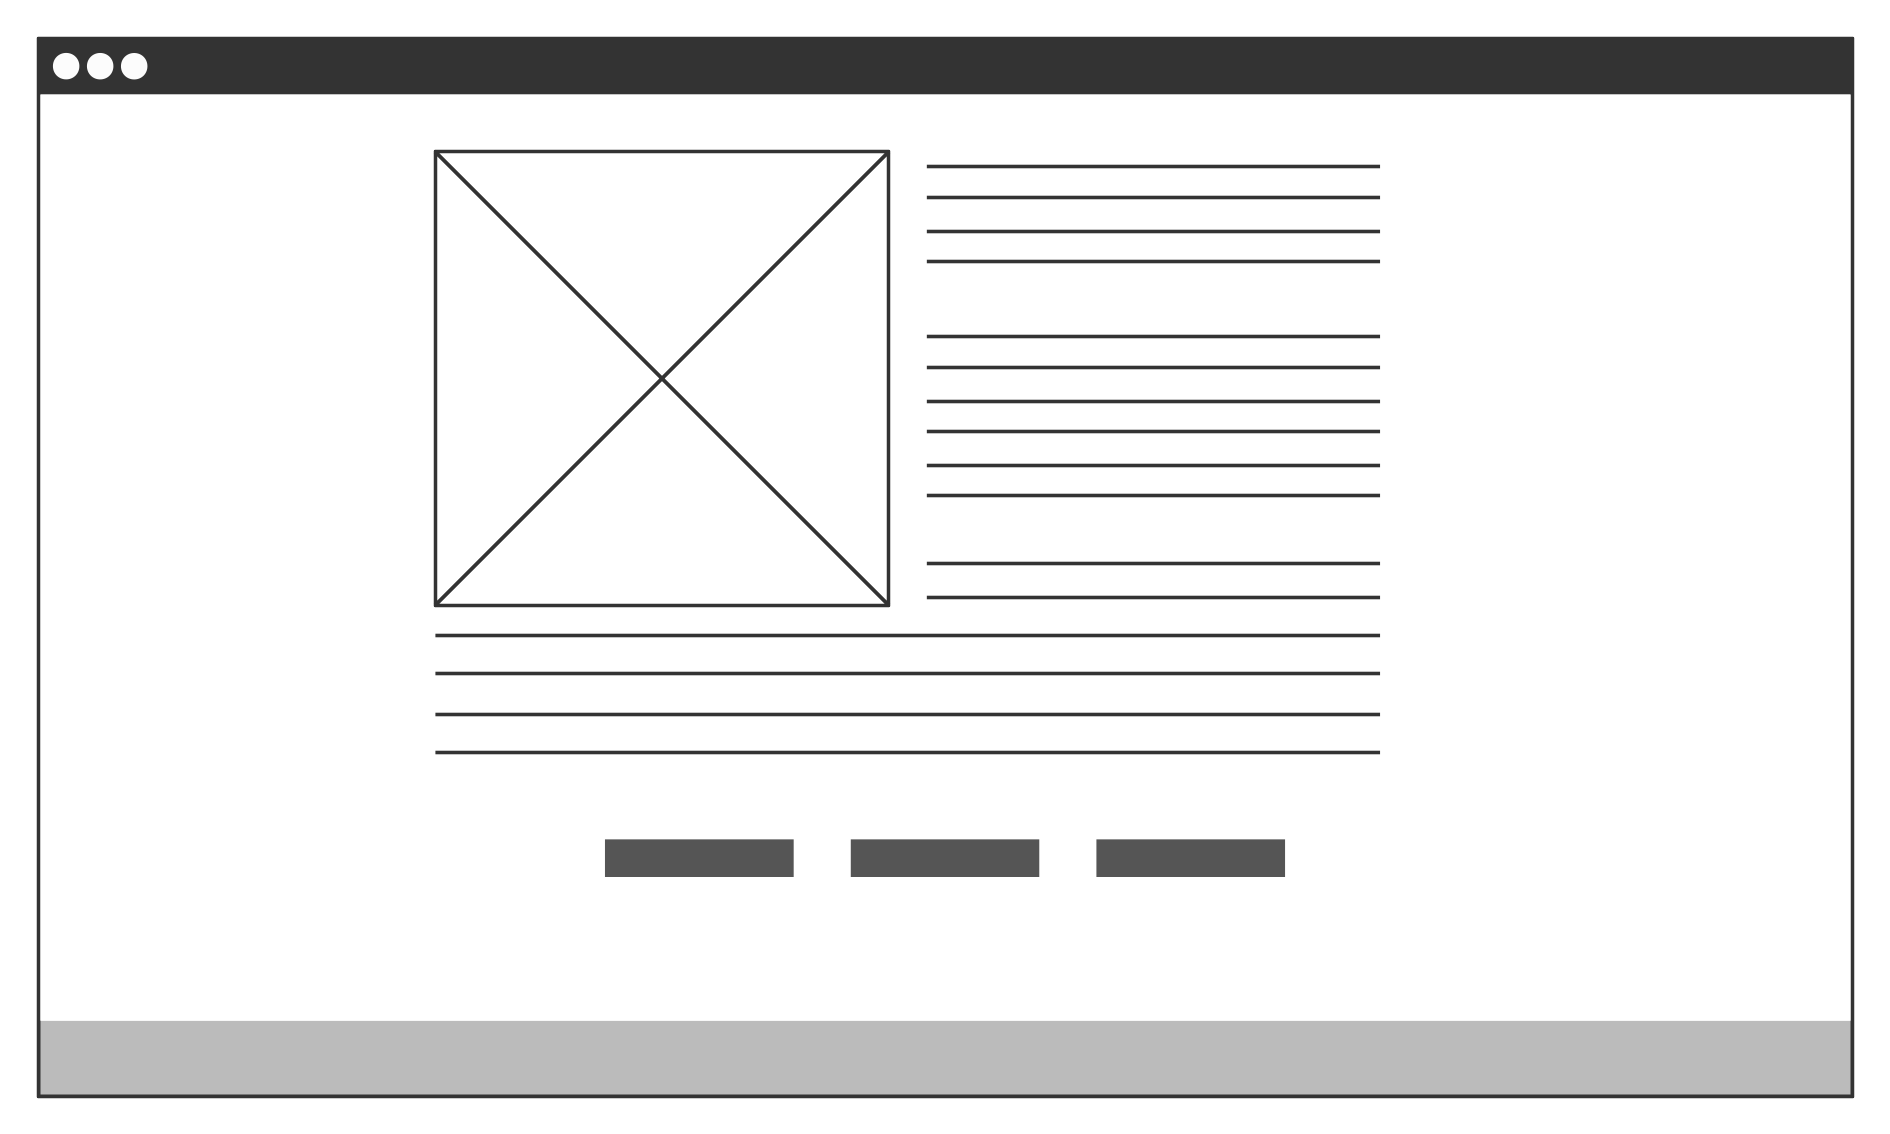
\includegraphics[width=.7\textwidth]{images/mockup.png}
    \caption{Screenshot. With some text to describe it.}
    \Description{A description for screen readers}
    \label{fig:mockup}
\end{figure}

\noindent\LaTeX:
\begin{Verbatim}[frame=single]
% places the figure here, or on top of the next page
\begin{figure}[ht]
    % centres the image on the page 
    \centering
    % load the image and set its width on the page
    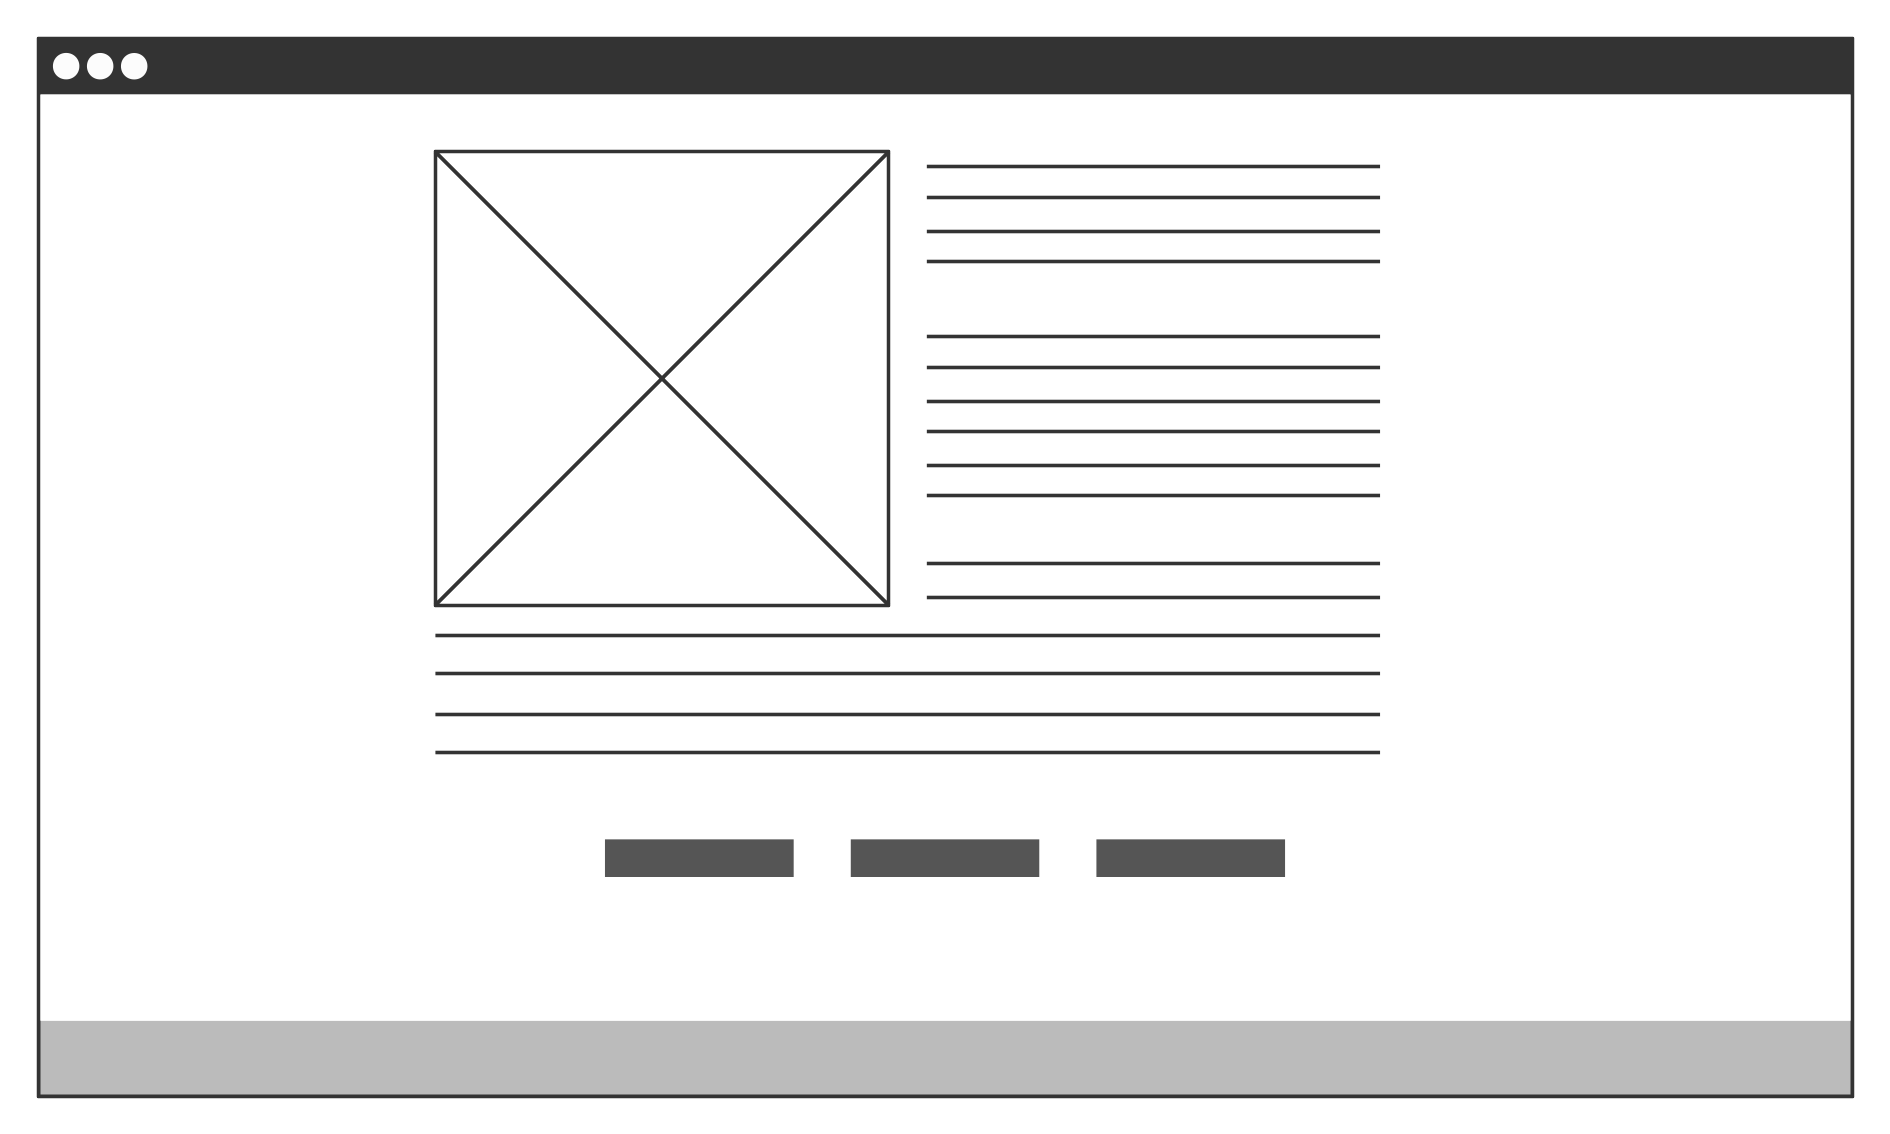
\includegraphics[width=.7\textwidth]{images/mockup.png}
    % add a caption
    \caption{Screenshot. With some text to describe it.} 
    \label{fig:mockup}
    \Description{A description for screen readers}
\end{figure}
\end{Verbatim}

\subsection*{Multiple images}

\begin{figure}[H]
    \centering
    \hspace{1cm}
    \begin{subfigure}{.35\textwidth}
        \centering
        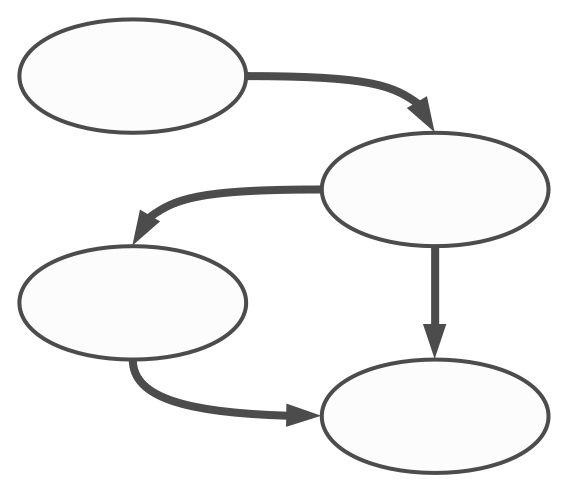
\includegraphics[width=\columnwidth]{images/flowchartA.png}
        \caption{Flowchart A.}~\label{fig:flowchart_a}
        \Description{A description for screen readers}
    \end{subfigure}
    \hfill
    \begin{subfigure}{.35\textwidth}
      \centering
        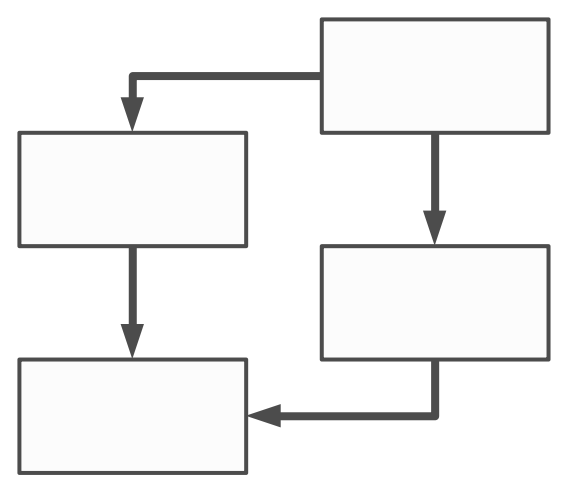
\includegraphics[width=\columnwidth]{images/flowchartB.png}
        \caption{Flowchart B.}~\label{fig:flowchart_b}
        \Description{A description for screen readers}
    \end{subfigure}
    \hspace{1cm}
    \caption{Flowchart for some processes.}~\label{fig:flowcharts}
\end{figure}

\noindent\LaTeX:
\begin{Verbatim}[frame=single]
\begin{figure}[ht]
    \centering
    % add some margin to the left
    \hspace{1cm}
    % insert sub-figure with specific width
    \begin{subfigure}{.35\textwidth}
        \centering
        % load image and make it fit the sub-figure width
        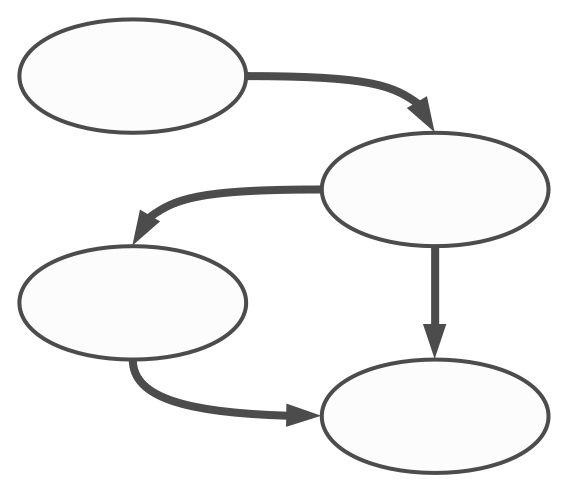
\includegraphics[width=\columnwidth]{images/flowchartA.png}
        \caption{Flowchart A.}~\label{fig:flowchart_a}
        \Description{A description for screen readers}
    \end{subfigure}
    % fill the space between images
    \hfill
    \begin{subfigure}{.35\textwidth}
      \centering
        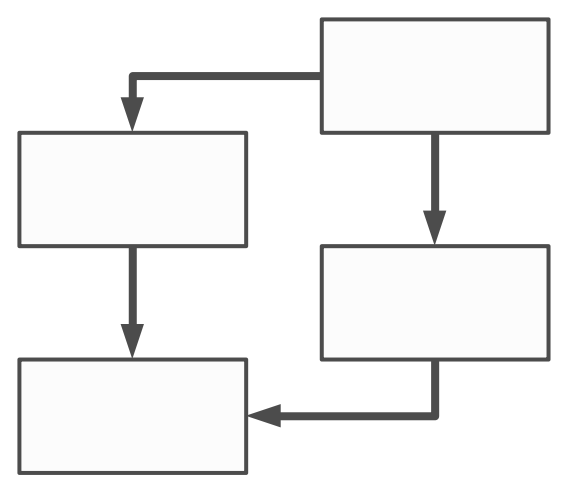
\includegraphics[width=\columnwidth]{images/flowchartB.png}
        \caption{Flowchart B.}~\label{fig:flowchart_b}
        \Description{A description for screen readers}
    \end{subfigure}
    % add some margin to the right
    \hspace{1cm}
    % caption for the set of images
    \caption{Flowchart for some processes.}~\label{fig:flowcharts}
\end{figure}
\end{Verbatim}

\section*{Tables}

\begin{table}[h]
    \centering
    \begin{tabular}{| l | c c | r |}
        \hline
        % place a row, each cell separated with &, finish the row with \\
        \textbf{A} & b & c & 1 \\ \hline
        % use \hline to add an horizontal line
        \textbf{X} & lorem & ipsum & 2 \\
        \textbf{S} & lor & \textit{em ispum} & 3.2 \\ \hline
    \end{tabular}
    \caption{Table of some properties}
    \label{tab:properties}
\end{table}

\noindent\LaTeX:
\begin{Verbatim}[frame=single]
\begin{table}[h]
    \centering
    % arrange the columns' alignment and vertical lines
    \begin{tabular}{| l | c c | r |}
        \hline
        % place a row, each cell separated with &, finish the row with \\
        \textbf{A} & b & c & 1 \\ \hline
        % use \hline to add an horizontal line
        \textbf{X} & lorem & ipsum & 2 \\
        \textbf{S} & lor & \textit{em ispum} & 3.2 
        \hline
    \end{tabular}
    \caption{Table of some properties}
    \label{tab:properties}
\end{table}
\end{Verbatim}

\section*{Equations}

\subsection*{Basic equations}

\begin{equation} \label{eq:my_equation}
    B = \sum_{\alpha \in A} \alpha \times \epsilon
\end{equation}

\noindent\LaTeX:
\begin{Verbatim}[frame=single]
\begin{equation} \label{eq:my_equation}
    B = \sum_{\alpha \in A} \alpha \times \epsilon
\end{equation}
\end{Verbatim}

\subsection*{Aligned equations}

\begin{align}
    X &= a^{\epsilon} \nonumber \\
    Z &= \frac{\sqrt{A \times B}}{\sum_{\gamma \in \Gamma} \gamma} 
    \label{eq:aligned_equation}
\end{align}

\noindent\LaTeX:
\begin{Verbatim}[frame=single]
% use &= to define the alignment
% use \nonumber to skip numbering the first equations
% \\ to get to a new line
% add label to last equation
\begin{align}
    X &= a^{\epsilon} \nonumber \\
    Z &= \frac{\sqrt{A \times B}}{\sum_{\gamma \in \Gamma} \gamma}
    \label{eq:aligned_equation}
\end{align}
\end{Verbatim}

\subsection*{Piecewise functions}

\begin{equation} \label{eq:equation_cases}
    x(r) =
        \begin{dcases*}
		a^2 + \sqrt{3} b & if $r$ is even \\
		a^2 + \frac{\sqrt{3}}{2} b & if $r$ is odd
		\end{dcases*}
\end{equation}

\noindent\LaTeX:
\begin{Verbatim}[frame=single]
\begin{equation} \label{eq:equation_cases}
    x(r) =
        \begin{dcases*}
        a^2 + \sqrt{3} b & if $r$ is even \\
        a^2 + \frac{\sqrt{3}}{2} b & if $r$ is odd
        \end{dcases*}
\end{equation}
\end{Verbatim}

\section*{Algorithms}

\begin{algorithm}
\caption{Euclidean Algorithm}\label{alg:euclid}
\begin{algorithmic}[1]
\Function{Euclid}{$a,b$}\Comment{Finding the GCD of $a$ and $b$}
\While{$b \neq 0$}
    \State $t \gets b$
    \State $b \gets a \mod b$
    \State $a \gets t$
\EndWhile
\State \textbf{return} $a$
\EndFunction
\end{algorithmic}
\end{algorithm}

\noindent\LaTeX:
\begin{Verbatim}[frame=single]
\begin{algorithm}
\caption{Euclidean Algorithm}\label{alg:euclid}
\begin{algorithmic}[1]
\Function{Euclid}{$a,b$}\Comment{Finding the GCD of $a$ and $b$}
\While{$b \neq 0$}
    \State $t \gets b$
    \State $b \gets a \mod b$
    \State $a \gets t$
\EndWhile
\State \textbf{return} $a$
\EndFunction
\end{algorithmic}
\end{algorithm}
\end{Verbatim}

\begin{algorithm}
\caption{My Algorithm}\label{alg:mine}
\begin{algorithmic}[1]
\Function{Custom}{$r,a,b$}\Comment{Implementing \cref{eq:equation_cases}}
\If{$r\ mod\ 2 \neq 0$}
    \State \textbf{return} $a^2 + \sqrt{3} b$
\Else
    \State \textbf{return} $a^2 + (\sqrt{3} / 2) b$
\EndIf
\EndFunction
\end{algorithmic}
\end{algorithm}

\noindent\LaTeX:
\begin{Verbatim}[frame=single]
\begin{algorithm}
\caption{My Algorithm}\label{alg:mine}
\begin{algorithmic}[1]
\Function{Custom}{$r,a,b$}\Comment{Implementing \cref{eq:equation_cases}}
\If{$r\ mod\ 2 \neq 0$}
    \State \textbf{return} $a^2 + \sqrt{3} b$
\Else
    \State \textbf{return} $a^2 + (\sqrt{3} / 2) b$
\EndIf
\EndFunction
\end{algorithmic}
\end{algorithm}
\end{Verbatim}

\section*{Code Listing}

\lstinputlisting[language=Python, 
    caption=Python example of GCD, 
    label={lst:gcd}]
    {code/gcd.py}

\noindent\LaTeX:
\begin{Verbatim}[frame=single]
% import code from gcd.py
% use parameters to set language, caption and label
\lstinputlisting[language=Python, 
    caption=Python example of GCD, 
    label={lst:gcd}]
    {code/gcd.py}
\end{Verbatim}

% adding language to code listing
\lstdefinelanguage{JavaScript}{
  keywords={abstract, any, as, boolean, break, case, catch, class, console, 
    const, continue, debugger, declare, default, delete, do, else, enum, export, 
    extends, false, finally, for, from, function, get, if, implements, import, in, 
    infer, instanceof, interface, keyof, let, module, namespace, never, new, null, 
    number, object, package, private, protected, public, readonly, require, return, 
    set, static, string, super, switch, symbol, this, throw, true, try, type, typeof, 
    undefined, unique, unknown, var, void, while, with, yield},
  morecomment=[l]{//},
  morecomment=[s]{/*}{*/},
  morestring=[b]',
  morestring=[b]",
  sensitive=true
}

\lstinputlisting[language=JavaScript, 
    caption=Helloworld in JavaScript, 
    label={lst:hello}]
    {code/hello.js}

\noindent\LaTeX:
\begin{Verbatim}[frame=single]
% adding language to code listing
\lstdefinelanguage{JavaScript}{
  keywords={abstract, any, as, boolean, break, case, catch, class, console, 
    const, continue, debugger, declare, default, delete, do, else, enum, 
    export, extends, false, finally, for, from, function, get, if, implements, 
    import, in, infer, instanceof, interface, keyof, let, module, namespace,
    never, new, null, number, object, package, private, protected, public, 
    readonly, require, return, set, static, string, super, switch, symbol, 
    this, throw, true, try, type, typeof, undefined, unique, unknown, var, 
    void, while, with, yield},
  morecomment=[l]{//},
  morecomment=[s]{/*}{*/},
  morestring=[b]',
  morestring=[b]",
  sensitive=true
}

\lstinputlisting[language=JavaScript, 
    caption=Helloworld in JavaScript, 
    label={lst:hello}]
    {code/hello.js}
\end{Verbatim}

\section*{Citing references}

Citing normally: \citep{alice2016}.

Citing the authors' names as part of the text: \citet{smith2018}.

Multiple citations: \citep{doe2015, alice2016}.

You can cite books, conference proceedings, articles, chapters, theses, websites, etc. \citep{paperpile2022}.

% using minipage to avoid pagebreak
\noindent\begin{minipage}[t]{\textwidth}
\renewcommand{\bibname}{References}
% \bibliographystyle{plainnat}
% using Harvard style
% \bibliographystyle{agsm}
% using ACM style
\bibliographystyle{ACM-Reference-Format}
% using APA style (requires apacite package)
% \bibliographystyle{apacite}
\bibliography{references}
\end{minipage}\\

\noindent\LaTeX:
\begin{Verbatim}[frame=single]
Citing normally: \citep{alice2016}.

Citing the authors' names as part of the text: \citet{smith2018}.

% note the alphabetical reordering
Multiple citations: \citep{doe2015, alice2016}.

% The commands for the list of references are set up by the template with 
% % list of references

\newpage
\renewcommand{\bibname}{References} % change name to References
% \phantomsection
% \addcontentsline{toc}{section}{References}

% using ACM style (defined in acm_settings.tex)
\bibliographystyle{ACM-Reference-Format}

% \bibliographystyle{plainnat}
% using Harvard style
% \bibliographystyle{agsm}

\bibliography{references}

% using APA style (requires apacite package)
% \bibliographystyle{apacite}
\end{Verbatim}

\noindent In \textit{references.bib} file:
\begin{Verbatim}[frame=single]
@article{smith2018,
    title = "Implementing X in Z context",
    author = "Smith, John J. and Doe, Jane",
    year = "2018",
    journal = "Transactions on this topic"
}
@inproceedings{doe2015,
    title = "Exploring Y",
    author = "Doe, Jane",
    year = "2015",
    booktitle = "Proceedings of that conference"
}
@book{alice2016,
    title = "Handbook of this method",
    author = "Alice, Bob",
    year = "2016",
    publisher = "Great Publisher"
}
% we use {\ } to avoid BibTex treating the string as last name and first name
@misc{paperpile2022,
    title = "The 14 BibTeX entry types",
    author = "Paperpile{\ }LLC",
    howpublished = "\url{https://www.bibtex.com/e/entry-types/}",
    year = "2022",
    note = "Accessed: 2025-08-29"
}
\end{Verbatim}

Examples of the most common types of entries, inspired from \href{https://www.bibtex.com/e/entry-types/}{bibtex.com/e/entry-types} and \href{https://bibtex.eu/types/}{bibtex.eu/types}.

\noindent \textbf{Article}, from journal, newspaper, etc.:
\begin{Verbatim}[frame=single]
@article{Citekey,
  author   = "Lastname, Firstname and Lastname, Firstname",
  title    = "Article Title",
  journal  = "Journal Name",
  year     = 2015,
  volume   = "Volume number",
  number   = "Issue number",
  pages    = "start page--end page",
}
\end{Verbatim}

\noindent \textbf{Book}, with edition and publisher information:
\begin{Verbatim}[frame=single]
@book{Citekey,
  author    = "Lastname, Firstname",
  title     = "Book Title",
  publisher = "Publisher Name",
  edition   = "Edition number",
  year      = 2020,
  address   = "Publisher address"
}
\end{Verbatim}

\noindent \textbf{InBook}, for particular chapters:
\begin{Verbatim}[frame=single]
@inbook{Citekey,
  author    = "Lastname, Firstname and Lastname, Firstname",
  title     = "Chapter title",
  booktitle = "Book title",
  editor    = "Lastname, Firstname",
  year      = 2016,
  publisher = "Publisher Name",
  address   = "Publisher address",
  pages     = "start page--end page"
}
\end{Verbatim}

\noindent \textbf{InProceedings}, for conference papers:
\begin{Verbatim}[frame=single]
@inproceedings{Citekey,
  author    = "Lastname, Firstname and Lastname, Firstname",
  title     = "Paper title",
  booktitle = "Proceeding name (conference edition)",
  series    = "Conference name",
  year      = 2010,
  pages     = "start page--end page",
  publisher = "Conference publisher, e.g., ACM or IEEE",
  address   = "Publisher address"
}
\end{Verbatim}

\noindent \textbf{MasterThesis} and \textbf{PhDThesis}, for student theses/dissertations:
\begin{Verbatim}[frame=single]
@phdthesis{Citekey,
  author  = "Lastname, Firstname",
  title   = "Thesis title",
  school  = "Institution name",
  address = "Institution address",
  year    = 2000,
  month   = jun
}
@mastersthesis{Citekey,
  author  = "Lastname, Firstname",
  title   = "Thesis title",
  school  = "Institution name",
  address = "Institution address",
  year    = 2008,
  month   = jun
}
% for a Bachelor's dissertation
@mastersthesis{Citekey,
  author  = "Lastname, Firstname",
  title   = "Thesis title",
  school  = "Institution name",
  address = "Institution address",
  year    = 2025,
  month   = jun,
  type    = "Bachelor's Dissertation"
}
\end{Verbatim}

\noindent \textbf{Misc}, for miscellaneous items, typically websites or blog entries:
\begin{Verbatim}[frame=single]
% for year use the date of publication,
% for note use the date you visited the website
% for author use the author name, website name or company name
@misc{Citekey,
    title        = "Page title",
    author       = "Lastname, Firstname",
    howpublished = "\url{https://www.}",
    year         = 2022,
    note         = "Accessed: date"
}
\end{Verbatim}

\section*{Cross referencing}

% using minipage to avoid pagebreak
\noindent\begin{minipage}[t]{\textwidth}
\section{Section}\label{cha:chapter_label}
\subsection{Subsection}\label{sec:section_label}
\end{minipage}~\\

In text, we can then point to \cref{cha:chapter_label} or \cref{sec:section_label}. Cross references are hyperlinks to the relevant section, images, etc.

The Cleverref package takes care of labelling items correctly, like \cref{fig:flowcharts}, \cref{tab:properties} or \cref{alg:euclid}. 

Cleverref also groups and orders references when you reference multiple items at once: \cref{eq:equation_cases,eq:aligned_equation,eq:my_equation}.

\noindent\LaTeX:
\begin{Verbatim}[frame=single]
% add labels to items you want to reference
\chapter{Chapter}\label{cha:chapter_label}
\section{Section}\label{sec:section_label}

In text, with can then point to \cref{cha:chapter_label} or 
\cref{sec:section_label}. 
Cross references are hyperlinks to the relevant section, images, etc.

The Cleverref package takes care of labelling items correctly, like 
\cref{fig:flowcharts}, \cref{tab:definitions} or \cref{alg:euclid}. 

Cleverref also groups and orders references when you reference multiple
items at once:
\cref{eq:equation_cases,eq:aligned_equation,eq:my_equation}.
\end{Verbatim}

\end{document}